\documentclass[titlepage, letterpaper, fleqn]{article}
\usepackage[utf8]{inputenc}
\usepackage{fancyhdr} % fancy headers, of course!
\usepackage{amsmath} % what do you think?
\usepackage{amsthm} % theorems!
\usepackage{extramarks} % more cute things
\usepackage{enumitem} % i'm not sure...
\usepackage{multicol} % multicolumn...?
\usepackage{amssymb} % more symbols
\usepackage{MnSymbol} % moar symbols?
\usepackage{booktabs} % cool looking tables
\usepackage{tikz} %venn and shizzle
\usepackage{mathrsfs} %math script for calligraphic scripting, I GUESS
\usepackage{listings}
\usepackage{mathtools}
\usepackage{graphicx}
\usepackage{subcaption}
\usepackage[draft, author=, mode=singleuser]{fixme}


\topmargin=-0.45in
\evensidemargin=0in
\oddsidemargin=0in
\textwidth=6.4in
\textheight=9.0in
\headsep=0.25in

\fxusetheme{colorsig} % theme for fixme
\fxsetface{margin}{\ttfamily\tiny}

\title{
\vspace{1in}
\textbf{Tecnológico de Monterrey} \\
\vspace{0.5in}
\textmd{Robotics} \\
\large{\textit{Dr. Ernesto Rodríguez Leal}} \\
\vspace{0.5in}
\textsc{Kinematic Analysis of a 3-RSP parallel mechanism}\\
\author{00783957 -- Alicia del Río \\
\and 00952040 -- Cristina Aparicio \\
\and 00822833 -- Guillermo Sotelo \\
\and 00809576 -- Sergio Sedas \\
\and 01170065 -- Xavier Sánchez}
\date{\today}
}

\DeclareMathOperator{\cose}{\mathcal{C}}
\DeclareMathOperator{\sen}{\mathcal{S}}

\begin{document}
\listoffixmes
\maketitle

\begin{abstract}
This paper presents a kinematic analysis of a 3-\underline{R}SP parallel mechanism.
The structure of the mechanism is formed by a fixed base and three identical legs of three links connected by a revolute, spherical and prismatic joints from base to top platform.
The paper includes forward and inverse position analysis, velocity and singularity analysis using screw theory, static and dynamic analysis, and the problems presented during the analysis phase for this particular configuration.
Results of motion simulation with SolidWorks are then compared with theoretical results obtained from Mathematica.
% \keywords{Parallel mechanism, RSP architecture, Forward kinematics, Inverse kinematics, Instantaneous screw axis, Jacobian matrix}
\end{abstract}


\section{Introduction}
\label{sec:intro}

A parallel mechanism consists of a series of links arranged in a closed kinematic chain connecting the base to the end-effector.
This type of configuration results in greater structural rigidity and accuracy than serial or open chain robots.
However, the drawback of this type of configuration is a smaller workspace due to link interference and greater complexity for analysis due to the closed kinematic loops of equations.
Nonetheless, parallel manipulators are the best alternative for applications requiring high load carrying capacity and precise positioning due to higher structural stiffness, reduced sensitivity to errors and built-in redundancy.
This paper focuses on the kinematics of a 3-\underline{R}SP mechanism with 3 degrees of freedom (DOF), where the R denotes a revolute joint which is actuated and fixed to the base, S denotes a spherical joint and P a prismatic joint connecting to the superior platform.

The paper is organized as follows:
\fxnote*{Arreglar secciones}{
Section~X contains a description of the mechanism's geometry.
Forward and inverse position analysis is presented in Section~X.
Section~X includes the velocity and singularity analysis using screw theory.
Static and dynamic analysis is described in Section~X.
Section~X details problems presented during the analysis phase for this particular configuration.}

%no debe haber espacio acá, sólo para que se vea qué porción es de quién
\fxwarning*{Hay que mover esto}{
Results of motion simulation with SolidWorks are compared with theoretical results obtained from Mathematica 11.0 using numerical examples for different positions of the platform.}

\section{Geometry}
\label{sec:geo}

The geometry of the 3-\underline{R}SP consists of a fixed base connected by three identical legs to a movable platform.
Each leg is comprised of three links where the first link is connected to the base by a revolute joint.
The second link is then connected to the first link by a spherical joint.
The third link is the platform connected to the second link by a prismatic joint.
The resulting geometry is the chain of RSP joints of the mechanism.
The actuated joints are the revolute joints (hence, the underlining in the text).
Fig.~\ref{fig:3dmodel} shows the 3D model of the mechanism.

\begin{figure}[htbp]
    \centering
    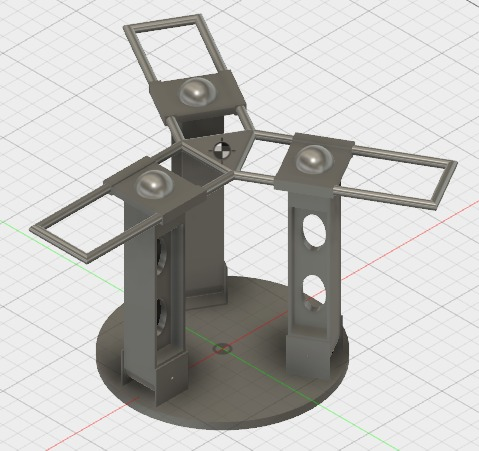
\includegraphics[width=0.75\textwidth]{fig_3dmodel}
    \caption{The 3-RSP mechanism 3D model}
    \label{fig:3dmodel}
\end{figure}

A schematic drawing of leg $i$ ($i = 1, 2, 3$) is shown in Fig.~\ref{fig:schema}.
The subscripts $i_j$ denote joint $j ( j = 1, 2, 3, 4, 5)$ in leg $i$.
The spherical joint is represented as three revolute joints:
one for each orthogonally intersecting axis of movement ($x, y, z$).
The revolute joints are equally distributed on the base and the locations are defined by vector $a_i$, going from the center of the base to the center of revolute joint $i$.
The spherical and prismatic joints are coincident at some point. The vector going from the revolute joint to this coincident point is denoted as $d_i$.
The axes of the prismatic joints intersect at the center of the platform.
The vector going from the center of the platform to the center of the sphere is the vector $b_i$.
Vector $p$ defines the position from the center of the base to the center of the platform.
The notation used is quite similar as the one used in~\cite{Rodriguez-Leal11}.

\begin{figure}[htbp]
    \centering
    \begin{subfigure}[b]{0.45\textwidth}
        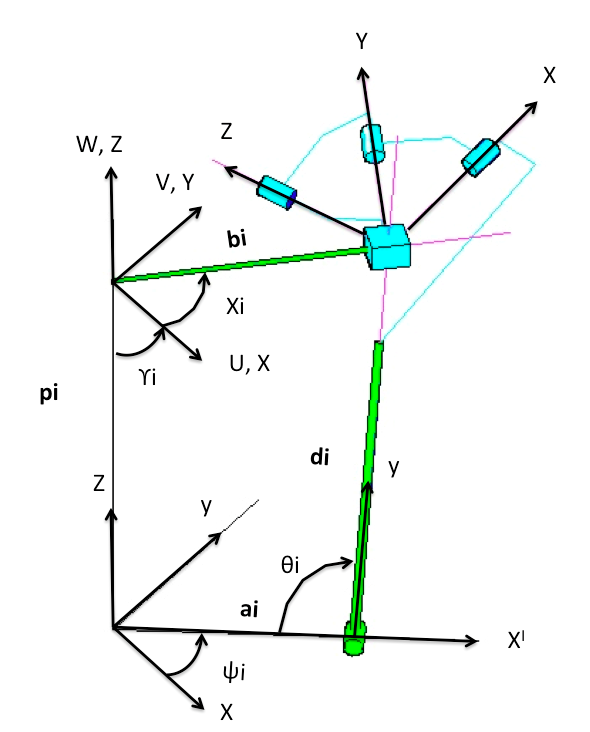
\includegraphics[width=\linewidth]{fig_schema_a}
    \end{subfigure}
    \begin{subfigure}[b]{0.45\textwidth}
        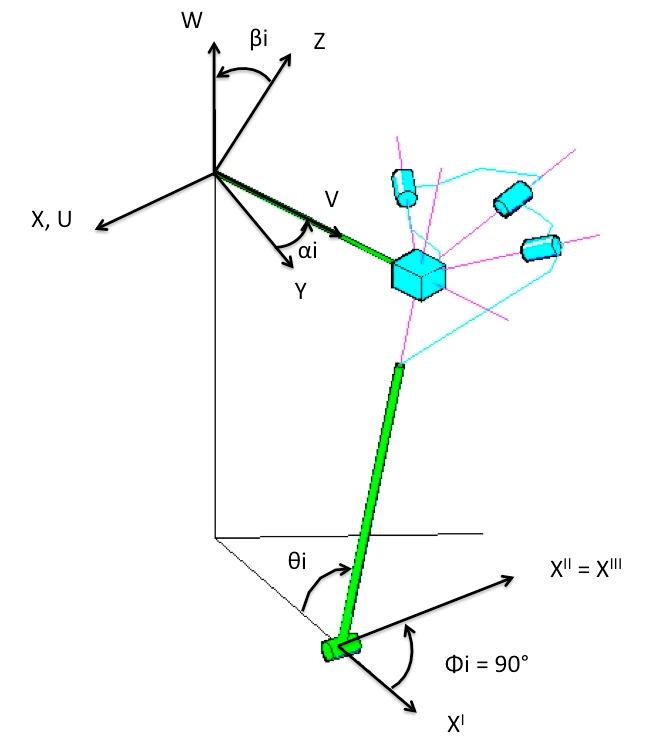
\includegraphics[width=\linewidth]{fig_schema_b}
    \end{subfigure}
    \caption{Schematic drawing for the $i$-th leg.}
    \label{fig:schema}
\end{figure}

\section{Analysis}
\label{sec:analysis}

Since the mechanism is comprised of three identical legs, the position and orientation of the platform can be obtained from the study of only one of them. A position analysis of the platform is performed and geometrical constraints applied to the closed loop equation.

The closed loop equation for leg $i$ can be written as

\begin{equation}
\label{eq:closed_loop}
    p + b_i = a_i + d_i
\end{equation}

where \fxnote{fill these placeholders}

\begin{equation}
    \label{eq:p}
    \mathbf{p} = [p_x, p_y, p_z]^T
\end{equation}

\begin{equation}
    \label{eq:a}
    \mathbf{a}_i = \mathbf{R}(Z,\psi_i) \cdot [a_i,0,0]^T
\end{equation}

\begin{equation}
    \label{eq:b}
    \mathbf{b}_i = \mathbf{R}(Z,\chi_i) \cdot \mathbf{R}(Z,\gamma_i) \cdot \mathbf{R}(T,\beta_i) \cdot [0, b_i, 0]^T
\end{equation}

\begin{equation}
    \label{eq:d}
    \mathbf{d}_i = \mathbf{R}(Z,\psi_i) \cdot \mathbf{R}(Z',\phi) \cdot \mathbf{R}(X'',\theta_{i}) \cdot [0, d_i, 0]^T
\end{equation}

The rotation matrices in Eq.~\ref{eq:a}, \ref{eq:b} and \ref{eq:d} are

\begin{equation}
    \label{eq:rot_Zpsi}
    \mathbf{R}(Z,\psi_i) =
    \begin{bmatrix}
        \cose\psi_i & -\sen\psi_i & 0 \\
        \sen\psi_i & \cose\psi_i & 0 \\
        0 & 0 & 1
    \end{bmatrix}
\end{equation}

\begin{equation}
    \label{eq:rot_Zphi}
    \mathbf{R}(Z,\phi_i) =
    \begin{bmatrix}
        \cose\phi_i & -\sen\phi_i & 0 \\
        \sen\phi_i & \cose\phi_i & 0 \\
        0 & 0 & 1
    \end{bmatrix}
\end{equation}

\begin{equation}
    \label{eq:rot_Xtheta}
    \mathbf{R}(X,\theta_i) =
    \begin{bmatrix}
        1 & 0 & 0 \\
        0 & \cose\theta_{i} & -\sen\theta_{i} \\
        0 & \sen\theta_{i} & \cose\theta_{i}
    \end{bmatrix}
\end{equation}

\begin{equation}
    \label{eq:rot_Zchi}
    \mathbf{R}(Z,\chi_i) =
    \begin{bmatrix}
    \cose\chi_i & -\sen\chi_i & 0 \\
    \sen\chi_i & \cose\chi_i & 0 \\
    0 & 0 & 1
    \end{bmatrix}
\end{equation}

\begin{equation}
    \label{eq:rot_Xalpha}
    \mathbf{R}(X,\alpha) = 
    \begin{bmatrix}
    1 & 0 & 0 \\
    0 & \cose\alpha & -\sen \alpha \\
    0 & \sen\alpha & Cos \alpha
    \end{bmatrix}
\end{equation}

\begin{equation}
    \label{eq:rot_Ybeta}
    \mathbf{R}(Y,\beta) =
    \begin{bmatrix}
        \cose\beta & 0 & \sen\beta \\
        0 & 1 & 0 \\
        -\sen\beta & 0 &\cose\beta
    \end{bmatrix}
\end{equation}

\begin{equation}
    \label{eq:rot_Xgamma}
    \mathbf{R}(Z,\gamma) =
    \begin{bmatrix}
        \cose\gamma & -\sen\gamma & 0 \\
        \sen\gamma & \cose\gamma & 0 \\
        0 & 0 & 1
    \end{bmatrix}
\end{equation}

Substituting and performing the matrix multiplication gives

\begin{equation}
    \label{eq:a_substitute}
    \mathbf{a}_i =
    \begin{bmatrix}
    a_i \cose \psi_i \\
    a_i \sen \psi_i \\
    0
    \end{bmatrix}
\end{equation}

\begin{equation}
    \label{eq:b_substitute}
    \mathbf{b}_i =
    \begin{bmatrix}
    (\cose \beta \cose \gamma \cose \chi_i + (\cose \gamma \sen \alpha \sen \beta - \cose \alpha \sen \gamma)\sen \chi_i) b_i \\
    (\cose \beta \cose \chi_i \sen \gamma + (\cose \alpha \cose \gamma \ \sen \alpha \sen \beta \sen \gamma)\sen \chi_i) b_i \\
    (-\cose \chi_i \sen \beta + \cose \beta \sen \alpha \sen \chi_i) b_i
    \end{bmatrix}
\end{equation}

\begin{equation}
    \label{eq:d_substitute}
    \mathbf{d}_i =
    \begin{bmatrix}
    -d \cose \theta_i \cose \psi_i \\
    -d \cose \theta_i \sen \psi_i \\
    d \sen \theta_i
    \end{bmatrix}
\end{equation}

Based on the previous equations, the solution for vector $p_i$, which determines the position of the center of the platform, can be written as

\begin{equation}
    \label{eq:p_solution}
    \mathbf{p} = 
    \begin{bmatrix}
    (a-d \cose (\theta _i)) \cose (\psi _i)-(\cose (\beta ) \cose (\gamma ) \cose (\chi _i)+(\cose (\gamma ) \sen (\alpha ) \sen (\beta )-\cose (\alpha ) \sen (\gamma )) \sen (\chi _i)) b_i \\
     (a-d \cose (\theta _i)) \sen (\psi _i)-(\cose (\beta ) \cose (\chi _i) \sen (\gamma )+(\cose (\alpha ) \cose (\gamma )+\sen (\alpha ) \sen (\beta ) \sen (\gamma )) \sen (\chi _i)) b_i \\
     d \sen (\theta _i)+(\cose (\chi _i) \sen (\beta )-\cose (\beta ) \sen (\alpha ) \sen (\chi _i)) b_i
    \end{bmatrix}
\end{equation}

and the orientation of the platform is determined by

\begin{equation}
    \label{eq:alpha}
    \alpha = 
\end{equation}

\begin{equation}
    \label{eq:beta}
    \beta = 
\end{equation}

\begin{equation}
    \label{eq:gamma}
    \gamma =
\end{equation}

\subsection{Forward Kinematic Analysis}
\label{sub:fwd}

The forward kinematic problem consists of determining the position and orientation of the end-effector given the values for the joint variables of the robot.
In this particular case, for a parallel robot, the end-effector is considered as the center of the moving platform.
The problem was approached by analyzing the position and the orientation of the platform independently.
To determine the position a geometric approach was applied.
Since the platform of the robotic mechanism is a triangle, the Fermat-Torricelli point theorem was chosen in order to obtain the central point of the platform when we know the magnitude of $\theta_1, \theta_2$ and $\theta_3$~\cite{WeissteinFermat}.

\subsubsection{The Fermat-Torricelli Problem} % (fold)
\label{ssub:fermat_torricelli_theorem}

The Fermat-Torricelli point can be defined as the point $X$ which minimizes the sum of distances from the vertices $A, B, C$:

$$|AX| + |BX| + |CX|$$

Fig.~\ref{fig:fermat_problem} shows a graphical representation of this problem.

\begin{figure}[htbp]
    \centering
    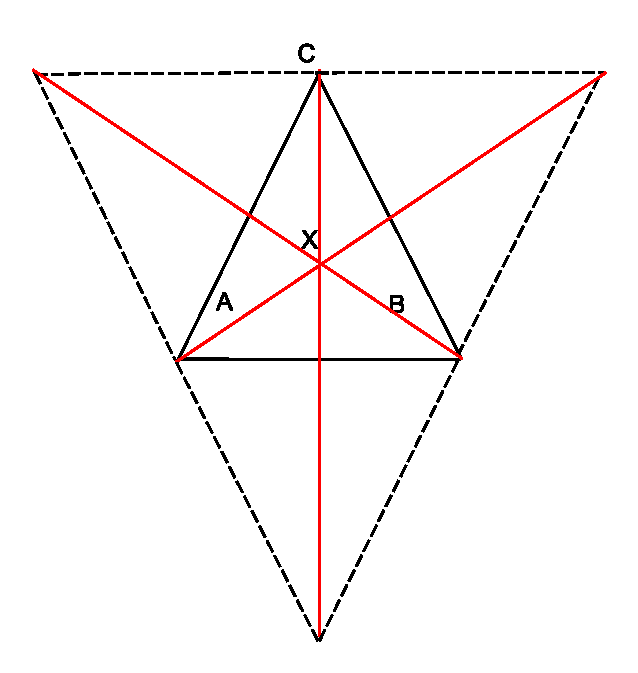
\includegraphics[width=0.7\textwidth]{fig_fermat}
    \caption{Graphical representation of the Fermat-Torricelli problem}
    \label{fig:fermat_problem}
\end{figure}


In this paper, this point was used to represent the center of the platform, that is to say point $p$ of equation~\ref{eq:p}.

In order to find this point an algebraic approach was used.
This approach is widely explained in~\cite{Palacios-Velez2015}, and it finds the $(x,y)$ coordinates of the point using the following equations:

%xFermat

%yFermat

where $xa, xb, xc$ represent the $x$ components of the vertices $A,B,C$ respectively, and $yc$ represents the $y$ component of the vertex $C$.

After obtaining the coordinates of the Fermat-Torricelli point on a 2-dimensional plane defined for this very purpose, the Fermat point was transformed into a 3-dimensional point which is referenced to the origin of the mechanism; the center of the base.

To transform the 2-dimensional point obtained into our 3-dimensional original plane, a cross product was performed between the $xFermat$ coordinate and the vector $q_{21}$, which is the unit vector from the spherical joint 1 to the spherical joint 2.

%xFvector

To obtain the $y$ component it's necessary to find a perpendicular vector to $q_{21}$.
The normalized cross product of vector $q_{21}$ and $q_{31}$ results into a normal vector to the platform.
If another cross product is performed with the vector $q_{21}$, a perpendicular vector to $q_{21}$ is obtained.

%q21 -> {-a+dCos[θ_1]+1/2(-a+dCos[θ_2]),1/2 √3(a-dCos[θ_2]),-dSin[θ_1]+dSin[θ_2]}


%q31 -> {-a+dCos[θ_1]+1/2(-a+dCos[θ_3]),-1/2 √3(a-dCos[θ_3]),-dSin[θ_1]+dSin[θ_3]}


Now a cross product between $yFermat$ coordinate and the vector obtained results into a vector from the spherical joint 1 which is perpendicular to vector $q_{21}$

%yFvector =

The sum of both vectors result into a vector from the spherical joint 1 and pointing to the center of the platform.
This is equal to vector $b$, but pointing in the opposite direction.
The final position of the center of the platform can be obtained by the sum of the vectors obtained, the $a$ and $d$ vectors of leg 1.
It's important to notice that these vectors are represented for leg 1.
If the vectors obtained with the Torricelli-Fermat analysis are summed
to the $a$ and $d$ vectors of another leg, the point obtained will not be the center of the platform but another point in space instead.

\begin{equation}
    \label{eq:p_Fermat}
    p = a_1 + d_1 + xFvector + yFvector
\end{equation}

Knowing the final position of the platform and the magnitude of the active joints, it is simple to obtain the orientation of the platform.
The equations for $\alpha, \beta$ and $\gamma$ can be obtained from Equation~\ref{eq:d}.

%alpha
%beta
%gamma



\bibliographystyle{splncs03}
\bibliography{biblio}

\end{document}